\documentclass[twoside,a4paper,11pt]{article}
\usepackage[T1]{fontenc}
\usepackage{times}
\usepackage{elcvia}
\usepackage{elcvia-submission}
\usepackage[english]{babel}
\usepackage{amsmath,amssymb}
\usepackage{graphicx}
\usepackage{booktabs}
\usepackage[numbers,sort&compress]{natbib}
\usepackage[hidelinks,breaklinks]{hyperref}
\usepackage{xurl}
\usepackage{placeins}
% Prevent isolated first or last paragraph lines at page breaks.
\clubpenalty=10000
\widowpenalty=10000
\renewcommand{\topfraction}{0.9}
\renewcommand{\bottomfraction}{0.8}
\renewcommand{\textfraction}{0.1}
\renewcommand{\floatpagefraction}{0.8}
\urlstyle{same}
% Break DOIs at their prefix separator, keeping identifier suffixes intact.
\newcommand{\doi}{doi: \begingroup\urlstyle{rm}%
  \def\UrlBreaks{\do\/}\def\UrlBigBreaks{\do\/}\Url}
\hypersetup{pdftitle={How Far Does Corruption Robustness Transfer? A Leave-One-Family-Out Study on CIFAR-100-C}}
\newif\ifblindreview
\ifdefined\ELCVIABlindReview\blindreviewtrue\else\blindreviewfalse\fi
\ifblindreview
\hypersetup{pdfauthor={}}
\else
\hypersetup{pdfauthor={Rakhman Seidigali and Yermakhan Khamitov}}
\fi

% Publication metadata, editor and received/accepted dates are intentionally unset.
\title{How Far Does Corruption Robustness Transfer?\\
A Leave-One-Family-Out Study on CIFAR-100-C\ifblindreview\else
\footnote[0]{Correspondence to: Rakhman Seidigali, \href{mailto:242171@astanait.edu.kz}{242171@astanait.edu.kz}.}\fi}
\author{Rakhman Seidigali and Yermakhan Khamitov\\[1ex]
\small\emph{School of Software Engineering, Astana IT University}\\
\small\emph{Astana, Kazakhstan}\\
\small\texttt{242171@astanait.edu.kz}\quad\texttt{242545@astanait.edu.kz}}
\date{}

\begin{document}
\ifblindreview\maketitleblind\else\maketitle\fi
\pagestyle{plain}
\raggedbottom
\noindent\hrulefill
\begin{abstract}
We test how corruption robustness transfers to an omitted family using 15 CIFAR-100-C types at five severities. We train four CIFAR-adapted ResNet-18 models from scratch, each withholding one family represented by Gaussian noise, defocus blur, fog, or JPEG compression. Compared with the primary clean-trained baseline on Metal Performance Shaders (MPS) with 32-bit floating-point (FP32) precision, held-out-family gains are 18.23, 12.24, 0.95, and 9.09 percentage points (pp) for Noise, Blur, Weather, and Digital. Ratios to the observed all-four gains are 0.45, 0.70, 0.14, and 0.88. Transfer is partial and varies by type: fog and brightness lose accuracy, while glass blur accounts for most of Blur's gain. The all-four control, trained with every representative, reaches 65.20\% mean corrupted accuracy against 47.83\% for the baseline, while its clean accuracy falls from 76.68\% to 72.68\%. These results use one training seed, with different random-number schedules and operator training frequencies across model cohorts.

\vspace{0.5cm}
\noindent\emph{Key Words}: Computer Vision, Image Classification, Corruption Robustness, Data Augmentation, Distribution Shift, Leave-One-Family-Out Evaluation.
\end{abstract}
\noindent\hrulefill

\section{Introduction}
Improved accuracy on training-related corruptions does not necessarily mean that a model will be robust to unseen distortions. Common-corruption benchmarks standardize evaluation~\cite{hendrycks2019corruptions}, but transfer depends on the similarity between augmentations and corruptions~\cite{geirhos2018generalisation,mintun2021interaction}. Recent CIFAR-100 experiments likewise show gains on some distortions and losses on others~\cite{trinh2024damp}, while model rankings can change with severity under continuous nuisance shifts~\cite{dunkel2025cns}.

We use a leave-one-family-out (LOFO) design to test transfer from three represented families to an excluded fourth. Overall corrupted accuracy can improve mainly through types explicitly used in augmentation. Holding out a family separates performance on trained operators from transfer to related types absent from augmentation. Family labels provide a reproducible omission rule, but shared visual effects make this an imperfect test of perceptual novelty~\cite{mintun2021interaction}. On CIFAR-100-C~\cite{hendrycks2019cifar100c}, our representatives are Gaussian noise, defocus blur, fog, and JPEG compression. Our three contributions are:
\begin{enumerate}
\item A representative-operator LOFO evaluation with a CIFAR-adapted ResNet-18 across six principal conditions.
\item Held-out-family gains and transfer ratios relative to the all-four control, measured across severity levels.
\item A comparison of all five augmented models by corruption type, including negative transfer and corruption types within represented families that were never used during training.
\end{enumerate}

\section{Related Work}
\subsection{Corruption benchmarks and evaluation}
ImageNet-C and CIFAR-100-C evaluate fixed transformations at five severities~\cite{hendrycks2019corruptions,hendrycks2019cifar100c}. Later work broadens evaluation with geometry-aware corruptions~\cite{kar2022common} and natural distribution shifts~\cite{hendrycks2021faces}. Gains on synthetic corruptions do not necessarily predict robustness to natural shifts~\cite{taori2020measuring}.

Recent benchmarks examine what fixed grids leave unmeasured. Shen et al.~\cite{shen2025continuous} index corruption effects by visual quality relative to human performance, revealing previously missed robustness gaps. CNS-Bench~\cite{dunkel2025cns} uses diffusion-model nuisance sliders and finds that model rankings change with shift magnitude. Its released levels and generators, which can vary shifts continuously, differ from CIFAR-C's pixel transformations. Our five-level grid measures neither continuous failure points nor transfer to natural shifts.

\subsection{Augmentation for robustness}
Policy learning~\cite{cubuk2019autoaugment} and the composition of transformations broaden augmentation coverage. AugMix~\cite{hendrycks2020augmix} regularizes stochastic mixtures for consistency, AugMax~\cite{wang2021augmax} optimizes these mixtures adversarially, and PRIME~\cite{modas2022prime} samples primitive transformations. DeepAugment operates through perturbed image-to-image networks~\cite{hendrycks2021faces}, while Patch Gaussian~\cite{lopes2019patch} adds noise to local patches. Their coverage and objectives differ from our one-operator, cross-entropy transfer study.

Recent work also changes augmentation composition and supervision. NoisyMix~\cite{erichson2024noisymix} combines noise in input and feature mixing with stability training, improving clean and corrupted CIFAR-100 performance. Heinonen et al.~\cite{heinonen2025mollification} couple noise and blur to degradation-dependent label smoothing; the effect on clean accuracy varies with the augmentation combination. Siedel et al.~\cite{siedel2026stylized} combine synthetic images, stylization, and TrivialAugment on CIFAR-100-C, but adding Mixup/CutMix can degrade performance. Augmentation diversity and composition therefore need to be evaluated together.

\subsection{Transfer to unseen corruptions and frequency effects}
Transfer is selective: Geirhos et al.~\cite{geirhos2018generalisation} report failures on untrained distortions, while tuned noise augmentation generalizes more broadly~\cite{rusak2020simple}. Mintun et al.~\cite{mintun2021interaction} link transfer to augmentation--corruption similarity and construct dissimilar corruptions on which gains weaken. Trinh et al.~\cite{trinh2024damp} compare direct augmentation with multiplicative weight perturbations using a train--test corruption matrix for ResNet-18 on CIFAR-100. Our four-family omission study examines a specific representative-operator setting within this established problem.

Frequency analyses also show the limits of family labels. Trade-offs between high- and low-frequency corruptions~\cite{yin2019fourier} motivate combining models with complementary frequency biases~\cite{saikia2021frequency}. Auxiliary Fourier-basis augmentation complements visual transformations~\cite{vaish2024fourier}. Family omission therefore does not by itself isolate frequency effects or perceptual novelty.

\section{Methodology}
\subsection{Data and corruption families}
CIFAR-100~\cite{krizhevsky2009tiny} contains 50,000 training and 10,000 test RGB images at $32\times32$ resolution in 100 classes. We use a saved, stratified seed-42 split: 45,000 images for fitting and 5,000 for clean validation, exactly 450 and 50 per class. The index sets are disjoint and cover the official training file. We evaluate on the official test file.

Let $\mathcal{F}=\{N,B,W,D\}$ denote Noise, Blur, Weather, and Digital, with corruption sets
\begin{align*}
\mathcal{C}_{N}&=\{\text{Gaussian noise, shot noise, impulse noise}\},\\
\mathcal{C}_{B}&=\{\text{defocus blur, glass blur, motion blur, zoom blur}\},\\
\mathcal{C}_{W}&=\{\text{snow, frost, fog, brightness}\},\\
\mathcal{C}_{D}&=\{\text{contrast, elastic transform, pixelate, JPEG compression}\}.
\end{align*}
These 15 primary types follow the CIFAR-C grouping~\cite{hendrycks2019corruptions}. We exclude the release's four additional types: Gaussian blur, saturate, spatter, and speckle noise. Five severities give 75 conditions per model, all using the same 10,000 test identities. We use the released Zenodo version 1 arrays~\cite{hendrycks2019cifar100c}.

\subsection{Representative-operator LOFO augmentation}
The fixed mapping is $r(N)=$ Gaussian noise, $r(B)=$ defocus blur, $r(W)=$ fog, and $r(D)=$ JPEG compression. We selected these operators for practical reasons: they provide a compact, reproducible design spanning the four categories. They apply additive noise, disk-kernel blur, a spatial fog field with intensity rescaling, and lossy compression, respectively. The mapping was not empirically optimized, and each representative covers only part of its family's mechanisms. For held-out family $F$, the allowed representatives are
\begin{equation}
\mathcal{R}_{-F}=\{r(G):G\in\mathcal{F},\ G\ne F\}.
\end{equation}
Table~\ref{tab:conditions} lists the conditions, and Figure~\ref{fig:design} shows LOFO-Noise. The model withholding $F$ receives no explicitly generated type from $\mathcal{C}_F$. It also receives no nonrepresentative types from the retained families, such as shot or impulse noise.

% Generated by paper/generate_assets.py from saved counts.
\begin{table}[htbp]
\caption{Six principal conditions. G, B, F, and J denote Gaussian noise, defocus blur, fog, and JPEG compression. One operator is sampled per corrupted presentation.}
\label{tab:conditions}
\centering
\setlength{\tabcolsep}{8pt}
\begin{tabular}{lcl}
\toprule
Condition & $p$ & Allowed representatives \\
\midrule
Primary clean & 0 & None \\
LOFO-Noise & 0.5 & B, F, J \\
LOFO-Blur & 0.5 & G, F, J \\
LOFO-Weather & 0.5 & G, B, J \\
LOFO-Digital & 0.5 & G, B, F \\
All-four control & 0.5 & G, B, F, J \\
\bottomrule
\end{tabular}
\end{table}


\begin{figure}[!htbp]
\centering
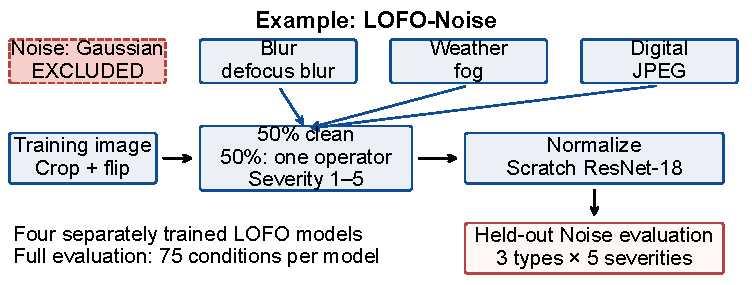
\includegraphics[width=0.76\textwidth]{figures/lofo_design.pdf}
\caption{LOFO-Noise design. Retained families supply one representative each. Four separate models exclude different families; every model receives the full 75-condition evaluation, including its held-out subset.}
\label{fig:design}
\end{figure}

We first apply a random $32\times32$ crop with padding 4 and a horizontal flip with probability 0.5. With probability $p=0.5$, we then choose an allowed operator and a severity from $\{1,\ldots,5\}$, both uniformly. Otherwise, we add no corruption. For branch indicator $Z$,
\begin{equation}
\Pr(Z=0)=1-p,\qquad
\Pr(Z=1,C=c,S=s)=\frac{p}{5|\mathcal{R}|}.
\end{equation}
Here $c\in\mathcal{R}$ and $s\in\{1,\ldots,5\}$. We apply one operator per corrupted presentation.

We adapt the CIFAR-specific reference code~\cite{cifarreference} and give each operator an explicit random generator. We clip and truncate its output to unsigned 8-bit RGB before tensor conversion. Appendix~\ref{app:records} gives the source commit and severity settings.

\subsection{Architecture and learning procedure}
We implement a CIFAR-adapted ResNet-18~\cite{he2016resnet} with torchvision and PyTorch~\cite{paszke2019pytorch}. It has $[2,2,2,2]$ basic blocks and a $3\times3$ input convolution with stride 1 and padding 1. We replace the initial max-pooling layer with identity and use a 100-way classifier. We train all 11,220,132 parameters from scratch.

We train for 100 epochs with batch size 128 and stochastic gradient descent: initial learning rate 0.1, momentum 0.9, and weight decay $5\times10^{-4}$. We disable Nesterov momentum and label smoothing. Cosine annealing uses $T_{\max}=100$ and $\eta_{\min}=0$, stepped at epoch end. After augmentation, we normalize FP32 RGB values in $[0,1]$ with mean $(0.5071,0.4867,0.4408)$ and standard deviation $(0.2675,0.2565,0.2761)$. Clean validation uses only tensor conversion and normalization. We minimize cross-entropy and select the first epoch with the highest clean-validation accuracy, using a strict-improvement rule.

\subsection{Accuracy and transfer ratio}
For model $m$, corruption $c$, severity $s$, and $n=10{,}000$ identities, percentage accuracy is
\begin{equation}
A_{m,c,s}=\frac{100}{n}\sum_{i=1}^{n}\mathbf{1}\{f_m(x_i^{c,s})=y_i\}.
\end{equation}
Family accuracy and overall corrupted accuracy are
\begin{equation}
A_{m,F}=\frac{1}{5|\mathcal{C}_F|}\sum_{c\in\mathcal{C}_F}\sum_{s=1}^{5} A_{m,c,s},\qquad
A_{m,\mathcal{C}}=\frac{1}{75}\sum_{F\in\mathcal{F}}\sum_{c\in\mathcal{C}_F}\sum_{s=1}^{5} A_{m,c,s}.
\end{equation}
We weight corruption types and severities equally: Noise contributes $3/15$ and each other family $4/15$. We report clean accuracy separately. The error $100-A_{m,\mathcal{C}}$ is unnormalized; mean corruption error (mCE) additionally normalizes errors against a reference model.

Let $m_{-F}$ omit family $F$, $m_0$ be the primary clean baseline, and $m_4$ the all-four control. We measure gain $\Delta_F$ in pp and compare it with the all-four gain using ratio $T_F$. A ratio of 0.70 means that the LOFO gain is 70\% as large as the all-four gain. We calculate both from unrounded scores:
\begin{equation}
\Delta_F=A_{m_{-F},F}-A_{m_0,F},\qquad
T_F=\frac{A_{m_{-F},F}-A_{m_0,F}}{A_{m_4,F}-A_{m_0,F}}.
\label{eq:transfer}
\end{equation}
The all-four score is not an upper bound on achievable robustness.

\section{Experimental Setup}
\subsection{Model cohorts and controls}
\label{sec:cohorts}
We compare seven completed 100-epoch runs. The four LOFO models used Apple Silicon MPS/FP32 with the legacy random-number-generation (RNG) schedule. Controlled-v2 added clean and all-four models on MPS/FP32; its clean model is the primary baseline. The historical clean baseline, trained with NVIDIA CUDA and automatic mixed precision (AMP) in Google Colab, is retained for reference only in Table~\ref{tab:overall} and Figure~\ref{fig:tradeoff}.

Legacy LOFO draws branch, operator, and severity choices from the worker's NumPy RNG, then uses Python's RNG to seed each operator's generator. Controlled-v2 draws from separate branch, operator, and severity streams on every image, including clean presentations. Its two runs load one shared initialization whose digest matches the LOFO records.

\subsection{Saved evaluations}
We evaluated the selected checkpoints in fixed inference mode with MPS/FP32, batch size 128, and the recorded normalization. We used no resizing, test-time augmentation, calibration, or adaptation. Saved results cover 380 conditions for the original five models and 152 for the controls: seven clean and 525 corrupted conditions. Comparing all 5.32 million saved predictions with official labels reproduced every count and aggregate. The saved histories confirm checkpoint selection. We build tables and plots from these counts.

\section{Results}
\subsection{Overall robustness and clean accuracy}
Table~\ref{tab:overall} and Figure~\ref{fig:tradeoff} show the trade-off across all seven models. All four LOFO models improve corrupted accuracy and lose clean accuracy. The all-four control has the highest corrupted accuracy, 65.20\%, at a clean-accuracy cost of 4.00 pp.

% Generated by paper/generate_assets.py from saved counts.
\begin{table}[htbp]
\caption{Seven completed seed-42 runs. Accuracy (\%); corrupted accuracy averages 75 conditions. Epoch is selected by clean validation. $h$: historical clean reference; $v$: controlled-v2; other rows: LOFO. Recorded cohorts are detailed in Appendix~\ref{app:records}.}
\label{tab:overall}
\centering
\setlength{\tabcolsep}{8pt}
\begin{tabular}{lrrr}
\toprule
Model & Epoch & Clean & Corrupted \\
\midrule
Historical clean$^{h}$ & 90 & 76.29 & 47.70 \\
Primary clean$^{v}$ & 94 & 76.68 & 47.83 \\
LOFO-Noise & 100 & 73.95 & 60.15 \\
LOFO-Blur & 100 & 72.28 & 63.48 \\
LOFO-Weather & 91 & 71.21 & 62.40 \\
LOFO-Digital & 95 & 73.87 & 64.99 \\
All-four control$^{v}$ & 98 & 72.68 & 65.20 \\
\bottomrule
\end{tabular}
\end{table}


\begin{figure}[!htbp]
\centering
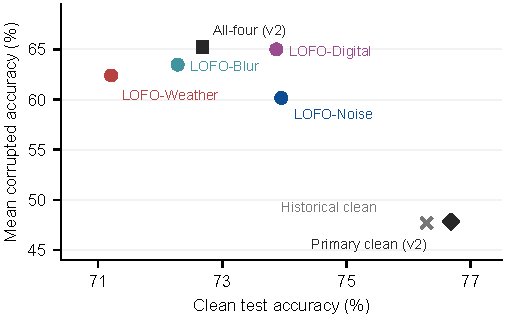
\includegraphics[width=0.61\textwidth]{figures/clean_vs_corrupted.pdf}
\caption{Clean versus mean corrupted accuracy. Circles: LOFO; diamond/square: controlled-v2 clean/all-four; cross: historical clean (reference only). Each point is one seed-42 run.}
\label{fig:tradeoff}
\end{figure}

LOFO-Digital scores 0.20 pp below all-four on corrupted data and retains more clean accuracy. With one seed, we cannot tell whether this 0.20 pp gap would persist across training seeds.

\subsection{Transfer to the excluded family}
Noise has the largest held-out-family gain and Weather the smallest (Table~\ref{tab:transfer}). The primary baseline also starts lowest on Noise.

% Generated by paper/generate_assets.py from saved counts.
\begin{table}[htbp]
\caption{Held-out-family accuracy (\%) and gain (pp) against the primary MPS/FP32 clean baseline. Each row uses a different LOFO network; the all-four model has explicit family exposure. Differences use unrounded measurements.}
\label{tab:transfer}
\centering
\setlength{\tabcolsep}{8pt}
\begin{tabular}{lrrrr}
\toprule
Family & Clean & LOFO & $\Delta$ (pp) & All-four \\
\midrule
Noise & 25.91 & 44.15 & +18.23 & 66.46 \\
Blur & 46.33 & 58.58 & +12.24 & 63.75 \\
Weather & 59.38 & 60.33 & +0.95 & 66.28 \\
Digital & 54.23 & 63.32 & +9.09 & 64.62 \\
\bottomrule
\end{tabular}
\end{table}


The transfer ratios order the families differently: Digital recovers 0.88 of the all-four family gain, compared with 0.14 for Weather. Noise improves substantially over clean training but remains furthest below its all-four score.

Table~\ref{tab:bootstrap} reports paired 95\% percentile intervals from 2,000 bootstrap resamples of the 10,000 test identities, retaining all types and severities and using common indices across models. The intervals reflect test-image sampling uncertainty only; they do not capture training-seed variability and are not significance tests. Weather's denominator interval, $[6.37,7.38]$ pp, stays away from zero.

% Generated by paper/paired_bootstrap.py; saved predictions only.
\begin{table}[!htbp]
\caption{Paired test-image bootstrap: 95\% percentile intervals, 2,000 resamples, seed 42. Each draw retains all types and five severities for each sampled identity across the LOFO, primary clean, and all-four models. Type gains use the indicated model; the denominator is the all-four family gain in Eq.~\ref{eq:transfer}.}
\label{tab:bootstrap}
\centering
\setlength{\tabcolsep}{5pt}
\begin{tabular}{lrrr}
\toprule
Family / type (model) & Gain (pp) & $T_F$ & Denominator (pp) \\
\midrule
Noise & [17.77, 18.73] & [0.44, 0.46] & [39.85, 41.23] \\
Blur & [11.75, 12.75] & [0.68, 0.73] & [16.85, 17.96] \\
Weather & [0.45, 1.43] & [0.07, 0.20] & [6.37, 7.38] \\
Digital & [8.67, 9.51] & [0.84, 0.91] & [9.90, 10.85] \\
\midrule
Glass blur (LOFO-Blur) & [30.71, 32.33] & --- & --- \\
Fog (LOFO-Weather) & [-8.80, -7.67] & --- & --- \\
Brightness (LOFO-Weather) & [-6.54, -5.22] & --- & --- \\
Contrast (LOFO-Weather) & [-6.22, -5.13] & --- & --- \\
\bottomrule
\end{tabular}
\end{table}


\subsection{Corruption-specific gains and negative transfer}
\label{sec:types}
All 15 held-out Noise cells improve (Figure~\ref{fig:heatmap}). Glass blur accounts for much of Blur's gain: it improves by 31.51 pp, while the mean gain across the other three Blur types is 5.82 pp.

\begin{figure}[!htbp]
\centering
% Use the available page width for the dense heatmap's labels and cell values.
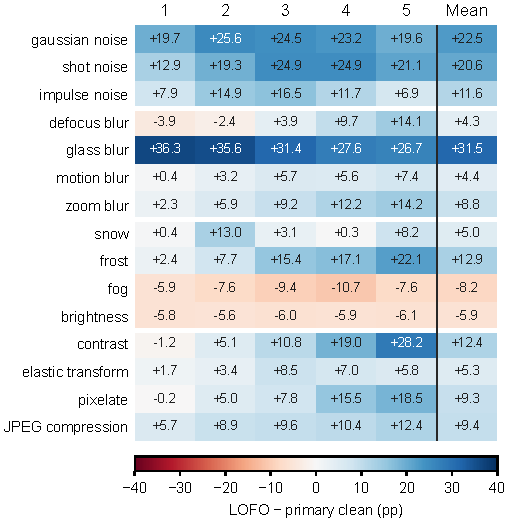
\includegraphics[width=0.90\textwidth]{figures/corruption_transfer_heatmap.pdf}
\caption{Held-out gains (pp) over the primary baseline by severity and their mean. Each row uses the model excluding its family; groups are Noise, Blur, Weather, and Digital. Red/blue denote negative/positive gains. Labels use exact-count rounding (half up).}
\label{fig:heatmap}
\end{figure}

Fog ($-8.23$ pp) and brightness ($-5.88$ pp) lose accuracy at every severity; snow and frost offset these losses in Weather's mean. All four Digital type means improve. Of the 75 held-out cells, 14 are negative: defocus at severities 1--2, all ten fog/brightness cells, and contrast and pixelate at severity 1.

% Keep the held-out heatmap with its discussion before the operator comparison.
\FloatBarrier
\subsection{Operator-level comparisons across augmented models}
\label{sec:operators}
Table~\ref{tab:operators} compares all five augmented models on every corruption type, including both represented and omitted families.

% Generated by paper/generate_assets.py from saved counts.
\begin{table}[!htbp]
\caption{Per-type gain (pp) over the primary clean baseline, averaged over five severities. Baseline accuracy is in \%. Bold: the LOFO model excluding that row's family. $^{*}$: training representative. N/B/W/D: Noise/Blur/Weather/Digital. Comparisons span the RNG schedules in Section~\ref{sec:cohorts}.}
\label{tab:operators}
\centering
\setlength{\tabcolsep}{4pt}
\begin{tabular}{lrrrrrr}
\toprule
Type & Baseline & LOFO-N & LOFO-B & LOFO-W & LOFO-D & All-four \\
\midrule
gaussian noise$^{*}$ & 21.27 & \textbf{+22.50} & +46.97 & +45.81 & +47.28 & +46.47 \\
shot noise & 29.52 & \textbf{+20.62} & +39.59 & +38.68 & +40.19 & +39.31 \\
impulse noise & 26.95 & \textbf{+11.58} & +35.30 & +35.66 & +36.41 & +35.88 \\
\addlinespace[3pt]
defocus blur$^{*}$ & 58.59 & +13.48 & \textbf{+4.25} & +10.96 & +13.96 & +12.06 \\
glass blur & 21.31 & +18.67 & \textbf{+31.51} & +32.95 & +24.67 & +31.50 \\
motion blur & 53.80 & +9.78 & \textbf{+4.45} & +7.66 & +9.66 & +9.01 \\
zoom blur & 51.63 & +17.90 & \textbf{+8.76} & +16.09 & +17.96 & +17.09 \\
\addlinespace[3pt]
snow & 53.97 & +6.05 & +5.52 & \textbf{+4.99} & +6.91 & +6.33 \\
frost & 48.13 & +13.76 & +16.15 & \textbf{+12.91} & +15.50 & +16.48 \\
fog$^{*}$ & 62.77 & +9.83 & +8.45 & \textbf{-8.23} & +10.56 & +8.47 \\
brightness & 72.67 & -2.43 & -4.01 & \textbf{-5.88} & -2.04 & -3.69 \\
\addlinespace[3pt]
contrast & 52.75 & +9.79 & +6.44 & -5.66 & \textbf{+12.38} & +7.97 \\
elastic transform & 60.21 & +4.88 & +1.85 & +3.68 & \textbf{+5.28} & +4.22 \\
pixelate & 52.26 & +12.23 & +13.26 & +13.27 & \textbf{+9.30} & +13.51 \\
JPEG compression$^{*}$ & 51.69 & +16.15 & +16.30 & +15.61 & \textbf{+9.41} & +15.86 \\
\bottomrule
\end{tabular}
\end{table}

% Present the comparison table before its detailed interpretation.
\FloatBarrier

\paragraph{Fog and contrast.}
Every model trained with fog improves contrast, while LOFO-Weather loses 5.66 pp on contrast and 8.23 pp on fog.

\paragraph{Brightness.}
All five augmented models lose brightness accuracy; even all-four loses 3.69 pp. LOFO-Weather has the largest loss, $-5.88$ pp.

\paragraph{Gaussian noise and glass blur.}
Models trained with Gaussian noise gain 35.30--36.41 pp on impulse noise, compared with 11.58 pp for LOFO-Noise. LOFO-Blur also gains 31.51 pp on glass blur without any explicit Blur augmentation.

\paragraph{Corruption types never used during training.}
For each LOFO model, the corruption types fall into three groups: all types in the excluded family, the three representatives used for augmentation, and the remaining types in represented families, which were never explicitly generated during training. The third group contains nine types for LOFO-Noise and eight for each other LOFO model. On these types, mean gains are 10.07, 14.26, 17.79, and 18.66 pp for LOFO-Noise, Blur, Weather, and Digital. For the last three models, these gains exceed their held-out-family gains, although the averages cover different type sets.

\subsection{Severity-dependent behavior}
The absolute gain in percentage points grows with severity for Blur (8.76 to 15.60 pp) and Digital (1.53 to 16.21 pp), while their accuracies decline (Figure~\ref{fig:severity}). Noise's gain rises from 13.49 pp at severity 1 to 21.98 pp at severity 3, then falls to 15.87 pp at severity 5. LOFO-Noise reaches 25.40\% at severity 5.

\begin{figure}[!htbp]
\centering
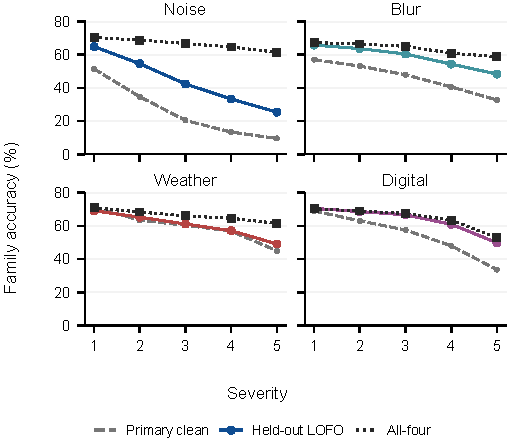
\includegraphics[width=0.66\textwidth]{figures/severity_transfer.pdf}
\caption{Family accuracy by severity, averaged over member types. Colored solid: held-out LOFO; gray dashed: primary clean; black dotted: all-four. Severity indices do not define a common physical scale across types.}
\label{fig:severity}
\end{figure}

Weather's gain is $-2.22$ pp at severity 1 and positive at severities 2--5, reaching +4.12 pp at severity 5. Snow and frost offset the fog and brightness losses.

\section{Discussion}
Noise improves across all three member types without explicit Noise augmentation. Its low baseline leaves more room for an absolute gain, but the gap to the all-four control shows that transfer is incomplete. Shared perturbation properties are a possible explanation~\cite{mintun2021interaction}, but our scores do not identify which properties the models learned.

The Gaussian-noise/glass-blur pattern agrees with Mintun et al.'s~\cite{mintun2021interaction} observation that glass blur's pixel permutations behave like noise. Models trained with JPEG also gain more on pixelate (12.23--13.51 pp) than LOFO-Digital (9.30 pp). These associations show why an omitted family is not necessarily visually dissimilar to the retained operators.

Fog adds a spatial field and rescales intensity. Shared intensity changes may help on contrast, but other operators, unequal exposure, and different RNG schedules prevent a causal interpretation. Frequency augmentation~\cite{vaish2024fourier} could help test this possibility. However, frequency shortcuts can improve performance on ImageNet-C and harm transfer to renditions~\cite{wang2025shortcuts}. Our scores do not identify a frequency mechanism.

Weather's small gain masks opposing effects: snow and frost improve, while fog and brightness deteriorate. A positive family mean therefore does not guarantee improvement on each member. Glass blur similarly dominates Blur's gain, obscuring smaller improvements on its other types. All five augmented models lose brightness accuracy. Trinh et al.~\cite{trinh2024damp} also report brightness losses with direct augmentation. This recurrence provides context but does not identify the cause in our models.

The cost in clean accuracy varies with the training recipe. NoisyMix~\cite{erichson2024noisymix} raises clean and corrupted CIFAR-100 accuracy, while multiplicative weight noise~\cite{trinh2024damp} improves robustness with little loss on clean data. Wiemann et al.'s 2026 preprint~\cite{wiemann2026interleaved} suggests gains from interleaved clean/noisy epochs. Mollification~\cite{heinonen2025mollification} and stylized synthetic augmentation~\cite{siedel2026stylized} do not always yield gains in both clean and corrupted accuracy when combined with other methods. Differences in models, data, losses, training budgets, and metrics prevent fair score rankings against our runs; matched controls are still needed.

\section{Limitations and Threats to Validity}
\label{sec:limitations}
\paragraph{Single-seed evidence and training budget.}
We completed one training seed, 42, per condition. The 75 conditions reuse the same test identities, so they do not establish variability across training seeds~\cite{bouthillier2021variance}. LOFO-Noise and LOFO-Blur selected epoch 100; this alone establishes neither convergence nor undertraining.

\paragraph{Cohorts, exposure, and exploratory timing.}
Legacy LOFO and controlled-v2 use different RNG schedules, and the initial LOFO tensors were not retained. At $p=0.5$, each shared operator is used with probability $1/6$ in LOFO and $1/8$ in all-four. We ran no ablation over $p$, so we cannot say how much of the 4.00 pp clean loss comes from $p=0.5$. These comparisons do not isolate operator effects. Pilot outcomes were known before the 29 October 2026 protocol freeze, and saved records cannot account for unlogged human decisions.

\paragraph{Dataset overlap.}
Exact-pixel hashing found four image contents shared between fitting and validation, eight between fitting and test, and two between validation and test. Some have conflicting labels; the split indices themselves are disjoint. Removing ten affected test identities changes primary gains by less than 0.006 pp and preserves their directions. Fitting/validation overlap may still affect checkpoint selection, and near-duplicates remain unchecked~\cite{barz2020duplicates}.

\paragraph{Representatives and scope.}
We study four representatives, one architecture, one split, and one $32\times32$ synthetic benchmark. Family effects overlap, and severity scales differ between operators. Five levels do not establish coverage across visual quality~\cite{shen2025continuous} or locate continuous nuisance-shift failure points~\cite{dunkel2025cns}. Generated training images may differ numerically from the released arrays. We measured neither frequency responses nor representation similarity, made no matched comparison with advanced augmentation methods, and did not test transfer to natural shifts~\cite{taori2020measuring}.

\section{Conclusion}
Training with representatives from three families improves the excluded family's mean accuracy in this measured setting. All four LOFO models exceed the primary MPS/FP32 baseline: Noise +18.23 pp, Blur +12.24 pp, Weather +0.95 pp, and Digital +9.09 pp. Transfer varies by type: fog and brightness lose accuracy, while glass blur improves strongly. The all-four control has the highest mean corrupted accuracy and lower clean accuracy. Cross-family gains therefore provide partial protection whose value depends on the corruption type. These results come from one seed with different RNG schedules and operator training frequencies. The next step is a multi-seed replication with a common RNG schedule and matched operator frequencies, to test whether the patterns persist under equal exposure before broadening representative coverage.

\section*{Data and Code Availability}
CIFAR-100 and CIFAR-100-C are available from their original sources~\cite{krizhevsky2009tiny,hendrycks2019cifar100c}. \ifblindreview Code and supporting materials will be identified upon acceptance.\else The public repository, \url{https://github.com/commedeschamps/cifar100c-lofo-robustness}, provides training/evaluation code, split indices, source snapshots, the frozen protocol, histories, and saved condition metrics. It also includes the figure/table generator, bootstrap analysis script, and derived assets.\fi\ Checkpoints and prediction caches are retained locally and are not publicly distributed.

% Keep the short declarations block together at the normal journal font size.
\par\noindent\begin{minipage}{\linewidth}
\section*{Declarations}
\noindent\textbf{AI assistance.} OpenAI Codex assisted with research code development, and computational verification. OpenAI ChatGPT and Anthropic Claude supported literature discovery and review. The authors retain responsibility for the reported results, references, and final text.

\noindent\textbf{Ethics.} This study uses existing, publicly available image-classification benchmarks without new participant recruitment.

\noindent\textbf{Author contributions (CRediT).} \ifblindreview Details withheld for anonymous review.\else R.S.: Conceptualization, Methodology, Software, Investigation, Validation, Formal analysis, Writing---original draft. Y.K.: Data curation, Writing---original draft, Writing---review \& editing, Visualization, Project administration.\fi

\noindent\textbf{Funding.} This research received no external funding.

\noindent\textbf{Competing interests.} The authors declare no competing interests.
\end{minipage}

\appendix
\section{Reproducibility details}
\label{app:records}
The MPS/FP32 records specify Python 3.14.5, PyTorch 2.14.1, torchvision 0.29.1, NumPy 2.5.4, OpenCV 5.0.0, and Pillow 13.0.0 on macOS 26.5.2 arm64, with two seeded, nonpersistent data-loader workers.

The five training severities follow the CIFAR-specific code~\cite{cifarreference} at commit \texttt{8190fe3}. Gaussian noise uses standard deviations $(0.04,0.06,0.08,0.09,0.10)$ on $[0,1]$. Defocus uses antialiased disk kernels with (radius, alias sigma) pairs $(0.3,0.4)$, $(0.4,0.5)$, $(0.5,0.6)$, $(1,0.2)$, and $(1.5,0.1)$. Fog uses a $32\times32$ diamond-square plasma map with (strength, decay) pairs $(0.2,3)$, $(0.5,3)$, $(0.75,2.5)$, $(1,2)$, and $(1.5,1.75)$. JPEG qualities are $(80,65,58,50,40)$.

The CIFAR-100-C version 1 archive has MD5 \texttt{11f0ed0f1191edbf9fa23466ae6021d3}. Receipts retain archive/array SHA-256 values, source/configuration identities, selection histories, and initialization digests. Controlled-v2 also retains its shared initializer.

\bibliographystyle{elcvia-numeric}
\bibliography{references}
\end{document}
